\section{Classical Runge-Kutta method}

\subsection{Description of Runge-Kutta}
As all other numerical solvers we have seen, Runge-Kutta discretizes the continous ODE by iteratively computing $x_{n+1}$ from $x_n$, i.e. using a finite-difference approximation. But whereas the previous methods take one long step from $x_n$ to $x_{n+1}$, Runge-Kutta is based on first taking multiple in-between steps $X_j$ for $j=1..s$ where $s$ is the number of stages. The computation $x_{n+1}$ is then computed as an weighted average of the stages. The higher number of stages, the higher is the order of the method and therefore also higher the accuracy. For error estimation instead of using step doubling, a higher order method is typically used ($\hat{x}_{n+1}$). The error is the estimated as $e_{n+1}=x_{n+1}-\hat{x}_{n+1}$. All in all the equations are denoted \cite{JrgensenRunge-KuttaEquations}:\\
\underline{Stages}

\begin{equation}
\label{eq:RKgeneral1}
\begin{aligned}
&T_{i}=t_{n}+c_{i} \Delta t_n \quad i=1,2, \ldots, s\\
&X_{i}=x_{n}+\Delta t_n \sum_{j=1}^{s} a_{i j} f\left(T_{j}, X_{j}\right) \quad i=1,2, \ldots, s
\end{aligned}
\end{equation}

Where the full \underline{next step} from $x_n$ to $x_{n+1}$ is calculated by

\begin{equation}
\label{eq:RKgeneral2}
\begin{aligned}
&t_{n+1}=t_{n}+\Delta t_n \\
&x_{n+1}=x_{n}+\Delta t_n \sum_{j=1}^{s} b_{j} f\left(T_{j}, X_{j}\right) \\
&\hat{x}_{n+1}=x_{n}+\Delta t_n \sum_{j=1}^{s} \hat{b}_{j} f\left(T_{j}, X_{j}\right) \\
&e_{n+1}=x_{n+1}-\hat{x}_{n+1}=\Delta t_n \sum_{j=1}^{s} d_{j} f\left(T_{j}, X_{j}\right) \quad d_{j}=b_{j}-\hat{b}_{j}
\end{aligned}
\end{equation}

The Explict and Implicit Euler methods are particular cases of the Runge-Kutta with s=1.

\\\

\textbf{Classical Runge-Kutta}\\
One intuitive idea is to let the stages only depend on previous $X_j$'s leading to Explicit Runge-Kutta methods. The Classical Runge-Kutta is such a method. Additionally, it is a 4 stage method where the different coefficients is chosen as summarized by this Butcher Tableau \cite{JrgensenRunge-KuttaEquations}

$$
\begin{array}{c|cccc}
0 & & & & \\
\frac{1}{2} & \frac{1}{2} & & & \\
\frac{1}{2} & 0 & \frac{1}{2} & & \\
1 & 0 & 0 & 1 & \\
\hline \mathrm{X} & \frac{1}{6} & \frac{1}{3} & \frac{1}{3} & \frac{1}{6}
\end{array}
$$

Which means that $x_{n+1}$ is iteratively calculated by

\begin{equation*}
\begin{array}{ll}
T_{1}=t_{n} & X_{1}=x_{n} \\
T_{2}=t_{n}+\frac{1}{2} \Delta t_n & X_{2}=x_{n}+\Delta t_n \frac{1}{2} f\left(T_{1}, X_{1}\right) \\
T_{3}=t_{n}+\frac{1}{2} \Delta t_n & X_{3}=x_{n}+\Delta t_n \frac{1}{2} f\left(T_{2}, X_{2}\right) \\
T_{4}=t_{n}+\Delta t_n & X_{4}=x_{n}+\Delta t_n f\left(T_{3}, X_{3}\right)
\end{array}
\end{equation*}

\begin{equation}
\label{eq:cRK1}
\begin{aligned}
&t_{n+1}=t_{n}+\Delta t_n \\
&x_{n+1}=x_{n}+\Delta t_n\left(\frac{1}{6} f\left(T_{1}, X_{1}\right)+\frac{1}{3} f\left(T_{2}, X_{2}\right)+\frac{1}{3} f\left(T_{3}, X_{3}\right)+\frac{1}{6} f\left(T_{4}, X_{4}\right)\right)
\end{aligned}
\end{equation}

The classical Runge-Kutta has no embedded method for error estimation.

\subsection{MATLAB implementation fixed step size}
The above mentioned classical Runge-Kutta method is implemented in MATLAB with a fixed step size $\Delta t_n = h$. For readability, the classical Runge-Kutta step is implemented separately in listing \ref{ERKpars} to be used in listing \ref{ERK} and \ref{ERKadapt}. The classical Runge-Kutta step is simply the implementation of equation \ref{eq:cRK1}.

\begin{adjustwidth*}{0cm}{-0.4cm}
\begin{lstlisting}[frame=single, language=Matlab,caption=Classical Runga-Kutta Step, label=ERKpars]
function [t1, x1] = ClassicalRungeKuttaStep(...
    fun,t,x,f,h,varargin)
h2 = 0.5*h;
alpha = h/6;
beta = h/3;

T1 = t;
X1 = x;
F1 = f;

T2 = x+h2;
X2 = x+h2*F1;
F2 = feval(fun,T2,X2,varargin{:});

T3 = T2;
X3 = x+h2*F2;
F3 = feval(fun,T3,X3,varargin{:});

T4 = t+h;
X4 = x+h*F3;
F4 = feval(fun,T4,X4,varargin{:});

t1 = T4;
x1 = x + alpha*(F1+F4) + beta*(F2+F3);
\end{lstlisting}
\end{adjustwidth*}

The classical Runge-Kutta with fixed step size is simply taking steps (listing \ref{ERKpars}) in the specified range as seen in listing \ref{ERK}.

\begin{adjustwidth*}{0cm}{-0.4cm}
\begin{lstlisting}[frame=single, language=Matlab,caption=Classical Runge-Kutta with fixed step size, label=ERK]
function [T,X] = ClassicalRungeKuttaFixedStep(...
    fun,tspan,x0,h,varargin)
% Integration interval
t0 = tspan(1);
tf = tspan(2);

% Initial conditions
t = t0;
x = x0;

T = t;
X = x';

%% Algo
while t < tf
    if (t+h > tf)
        h = tf-t;
    end
    % f at x_n
    f = feval(fun, t,x,varargin{:});

    % Take step of size h to obtain x_{n+1}
    [t, x] = ClassicalRungeKuttaStep(...
        fun,t,x,f,h,varargin{:});

     T = [T; t];
     X = [X; x'];
end
\end{lstlisting}
\end{adjustwidth*}



\subsection{MATLAB implementation adaptive step size}
Similarly to listing \ref{ERK}, the below implementation of an adaptive step size uses classical Runge-Kutta steps (listing \ref{ERKpars}) and adaptively changes the step size relative to specified tolerances. The error estimation is based on step doubling, iteratively decreasing the step size until the error (as estimated by taking the two half steps) is below specified tolerances. The step doubling procedure is described in full detail in Section \ref{sec:stepdoubling}. The implementation of the adaptive classical Runge-Kutta is seen in listing \ref{ERKadapt}.

\begin{adjustwidth*}{0cm}{-0.4cm}
\begin{lstlisting}[frame=single, language=Matlab,caption=Explicit Runge-Kutta with adaptive step size, label=ERKadapt]
function [T,X,H] = ClassicalRungeKuttaAdaptiveStep(...
    fun,tspan,x0,h0,abstol,reltol,varargin)
epstol = 0.8;
kpow = 0.2; % 1/(order+1)
facmin = 0.1;
facmax = 5;

% Integration interval
t0 = tspan(1);
tf = tspan(2);

% Initial conditions
t = t0;
h = h0;
x = x0;

H = h;
T = t;
X = x';

%% Algo
while t < tf
    if (t+h > tf)
        h = tf-t;
    end
    f = feval(fun, t,x,varargin{:});

    AcceptStep = false;
    while ~AcceptStep
        % Take step of size h
        [t1, x1] = ClassicalRungeKuttaStep(...
            fun,t,x,f,h,varargin{:});

        % Take step of size h/2
        hm=0.5*h;
        [tm, xm] = ClassicalRungeKuttaStep(...
            fun,t,x,f,h,varargin{:});
        
        fm = feval(fun,tm,xm,varargin{:});
        [t1hat, x1hat] = ClassicalRungeKuttaStep(...
            fun,tm,xm,fm,hm,varargin{:});

        % Error estimation
        e = x1hat-x1;
        r = max(abs(e) ./ max(abstol, abs(x1hat) .*reltol));

        AcceptStep = (r<=1.0);
        if AcceptStep
            t = t+h;
            x = x1hat;
              
            T = [T;t];
            X = [X;x'];
            H = [H;h]; % Save taken step sizes
        end
        % Asymptotic step size controller
        h = max(facmin,min((epstol/r)^kpow,facmax))*h;
    end
end
\end{lstlisting}
\end{adjustwidth*}

\subsection{Van der Pol}
Let us use the two numerical solvers for solving the Van der Pol problem defined as

\begin{equation}
\label{eq:vanderpol}
\begin{aligned}
&\dot{x}_{1}(t)=x_{2}(t) \\
&\dot{x}_{2}(t)=\mu\left(1-x_{1}(t)^{2}\right) x_{2}(t)-x_{1}(t)
\end{aligned}
\end{equation}


\subsubsection*{Fixed step size}
See Figure \ref{fig:5_4fix} for the solution using the fixed step size. Clearly there is an increasing precision for lowering the step size $h$. This is particularly the case for the stiff-problem ($\mu = 20$) where the solution quickly goes to $\infty$ for $h=0.1$.

\begin{figure}[htb]
    \centering
    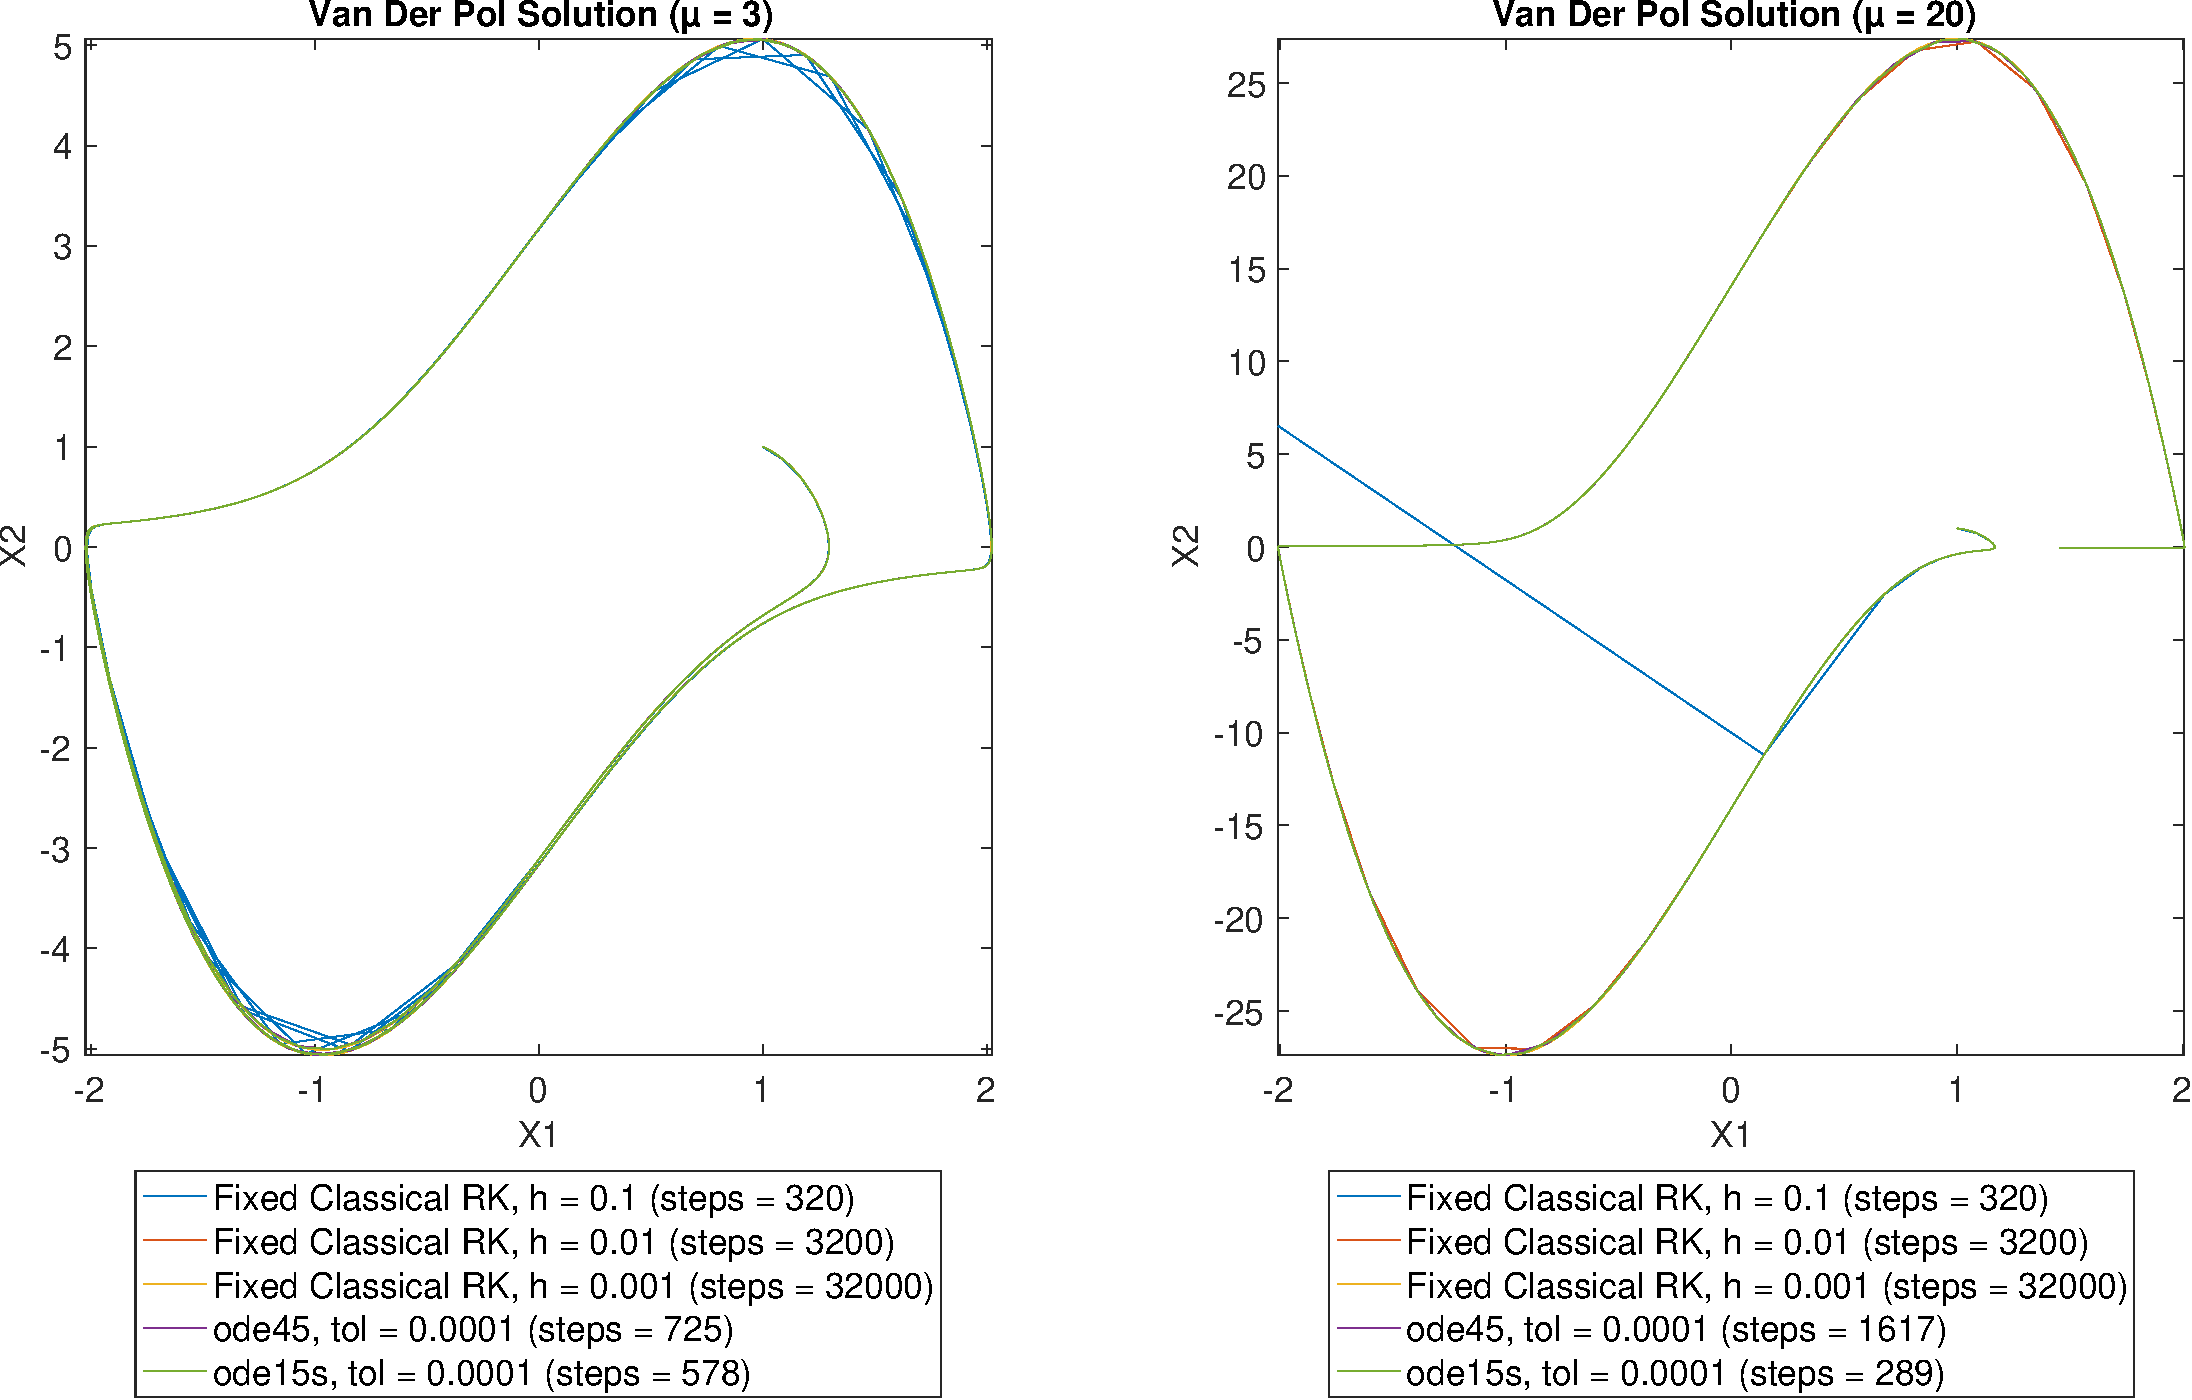
\includegraphics[width=\textwidth]{plots/5_4fix_a.pdf}
    \caption{Solution of Van der Pol using classical Runge-Kutta with fixed step size.}
    \label{fig:5_4fix}
\end{figure}







\subsubsection*{Adaptive step size}
The phase portrait of the solution from the solving the Van der Pol with the adaptive step size is seen in Figure \ref{fig:5_4}.

The corresponding $x_1$ and $x_2$ values over time is seen in Figure \ref{fig:5_4a}. Here, the stiffness of the problem with $\mu = 20$ is really clear. Interestingly, but not surprisingly, the step sizes drops accordingly to the stiff peaks of $x_2$ as seen in Figure \ref{fig:5_4b}.

\begin{figure}[h]
    \centering
    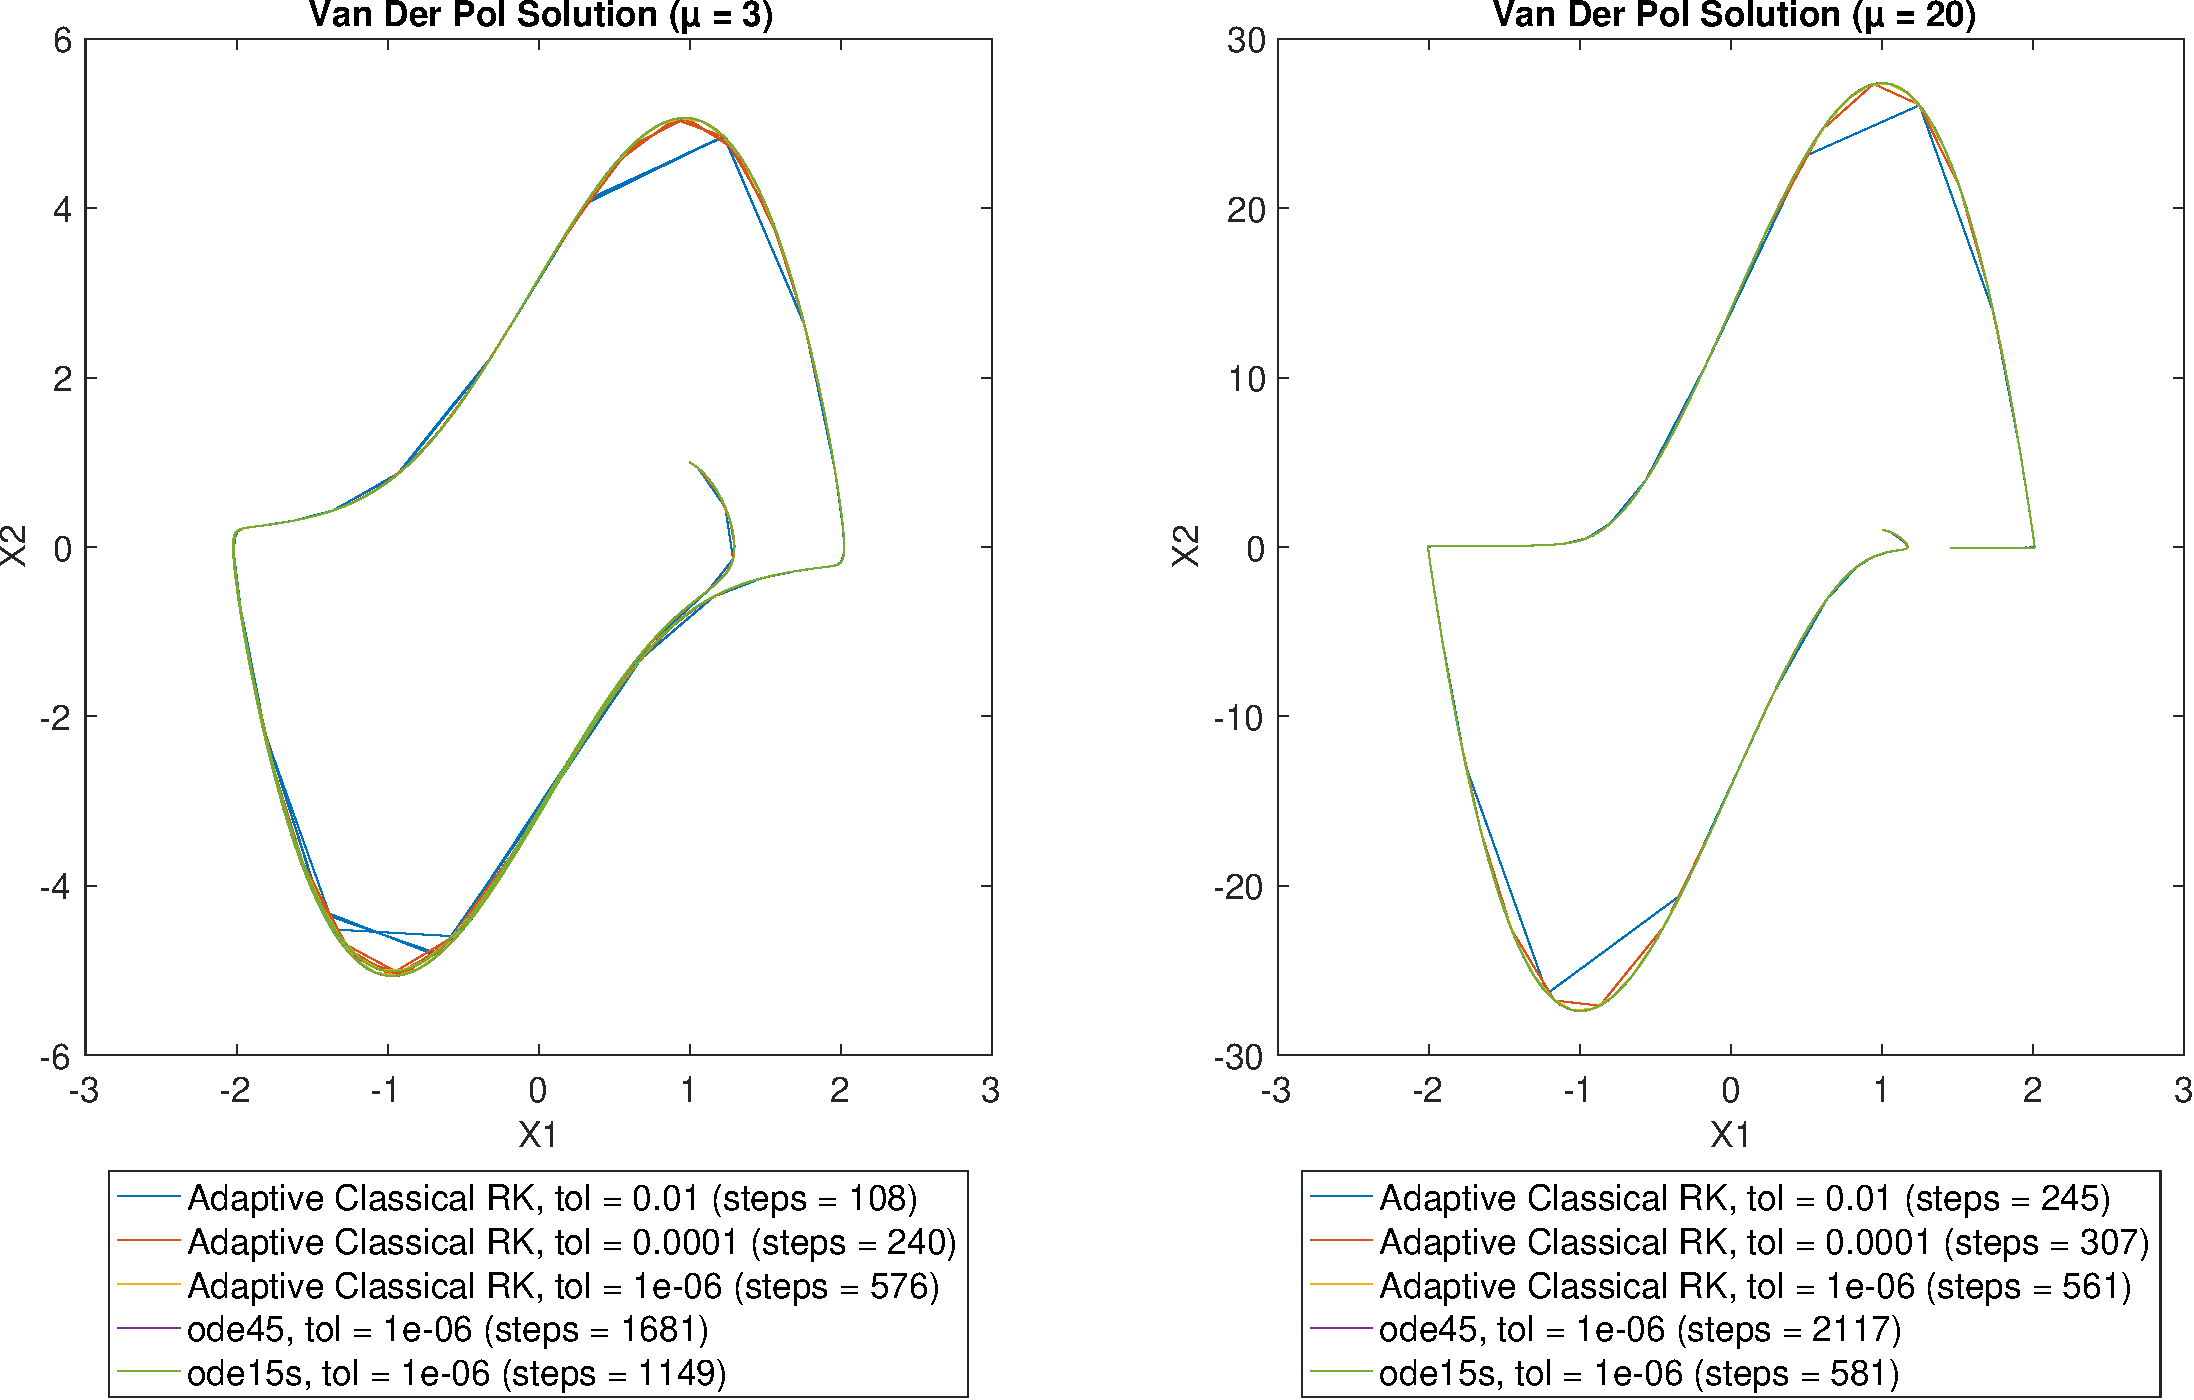
\includegraphics[width=\textwidth]{plots/5_4.pdf}
    \caption{Phase portrait of the solution of Van der Pol using classical Runge-Kutta with adaptive step size.}
    \label{fig:5_4}
\end{figure}






\begin{figure}[h]
\centering
\begin{subfigure}[b]{\textwidth}
   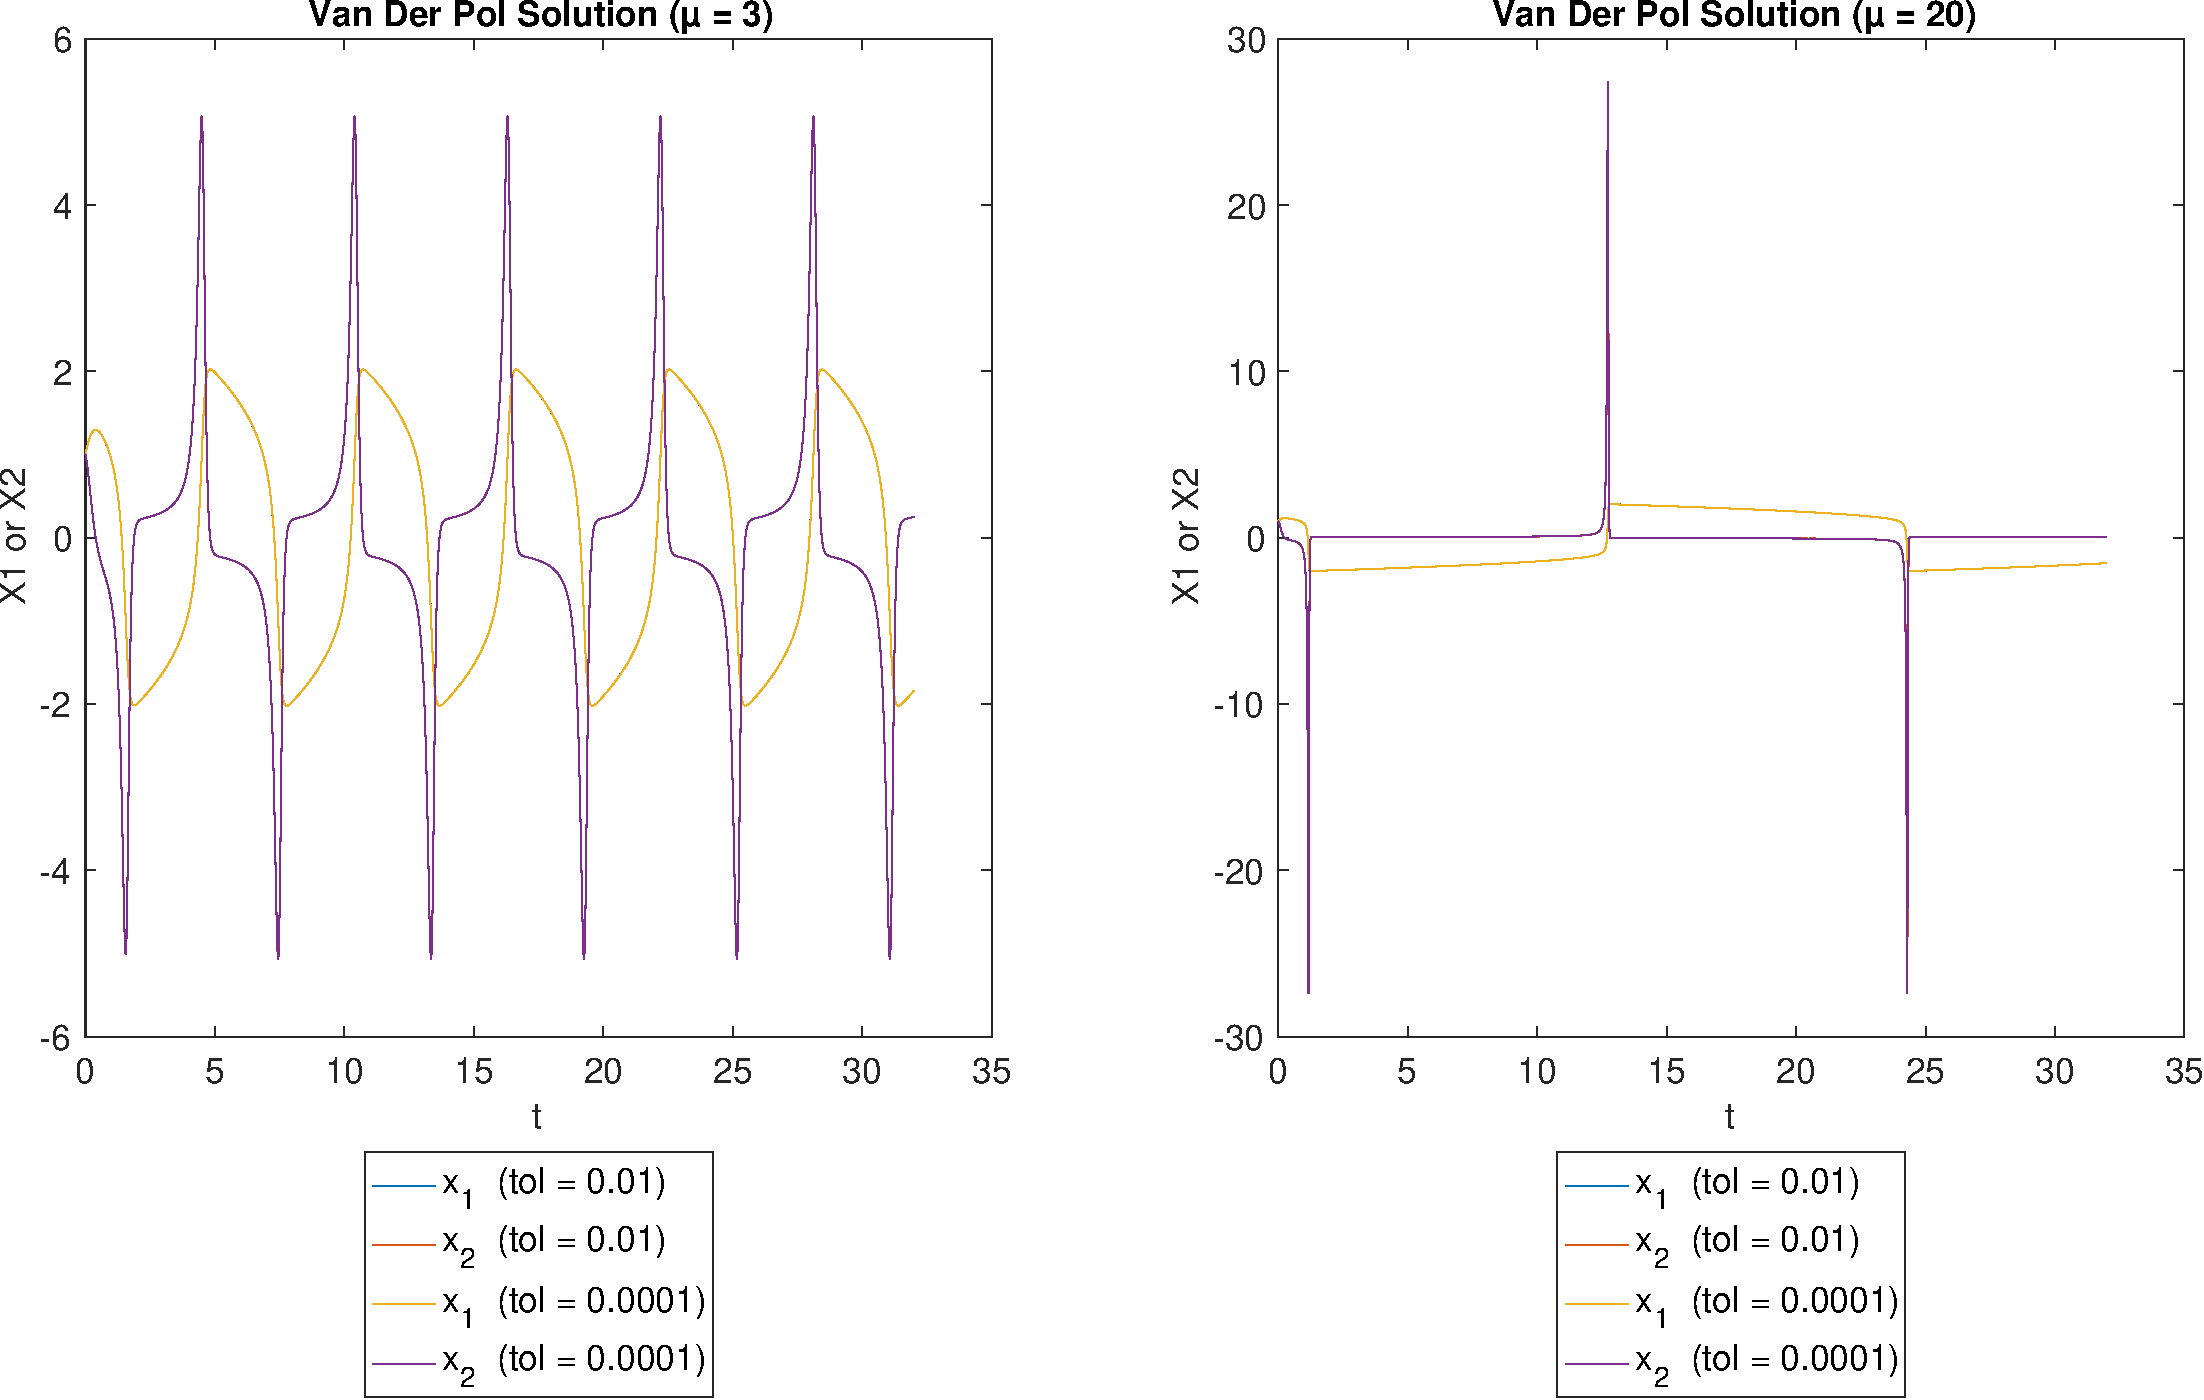
\includegraphics[width=1\linewidth]{plots/5_4a.pdf}
   \caption{}
   \label{fig:5_4a} 
\end{subfigure}

\begin{subfigure}[b]{\textwidth}
   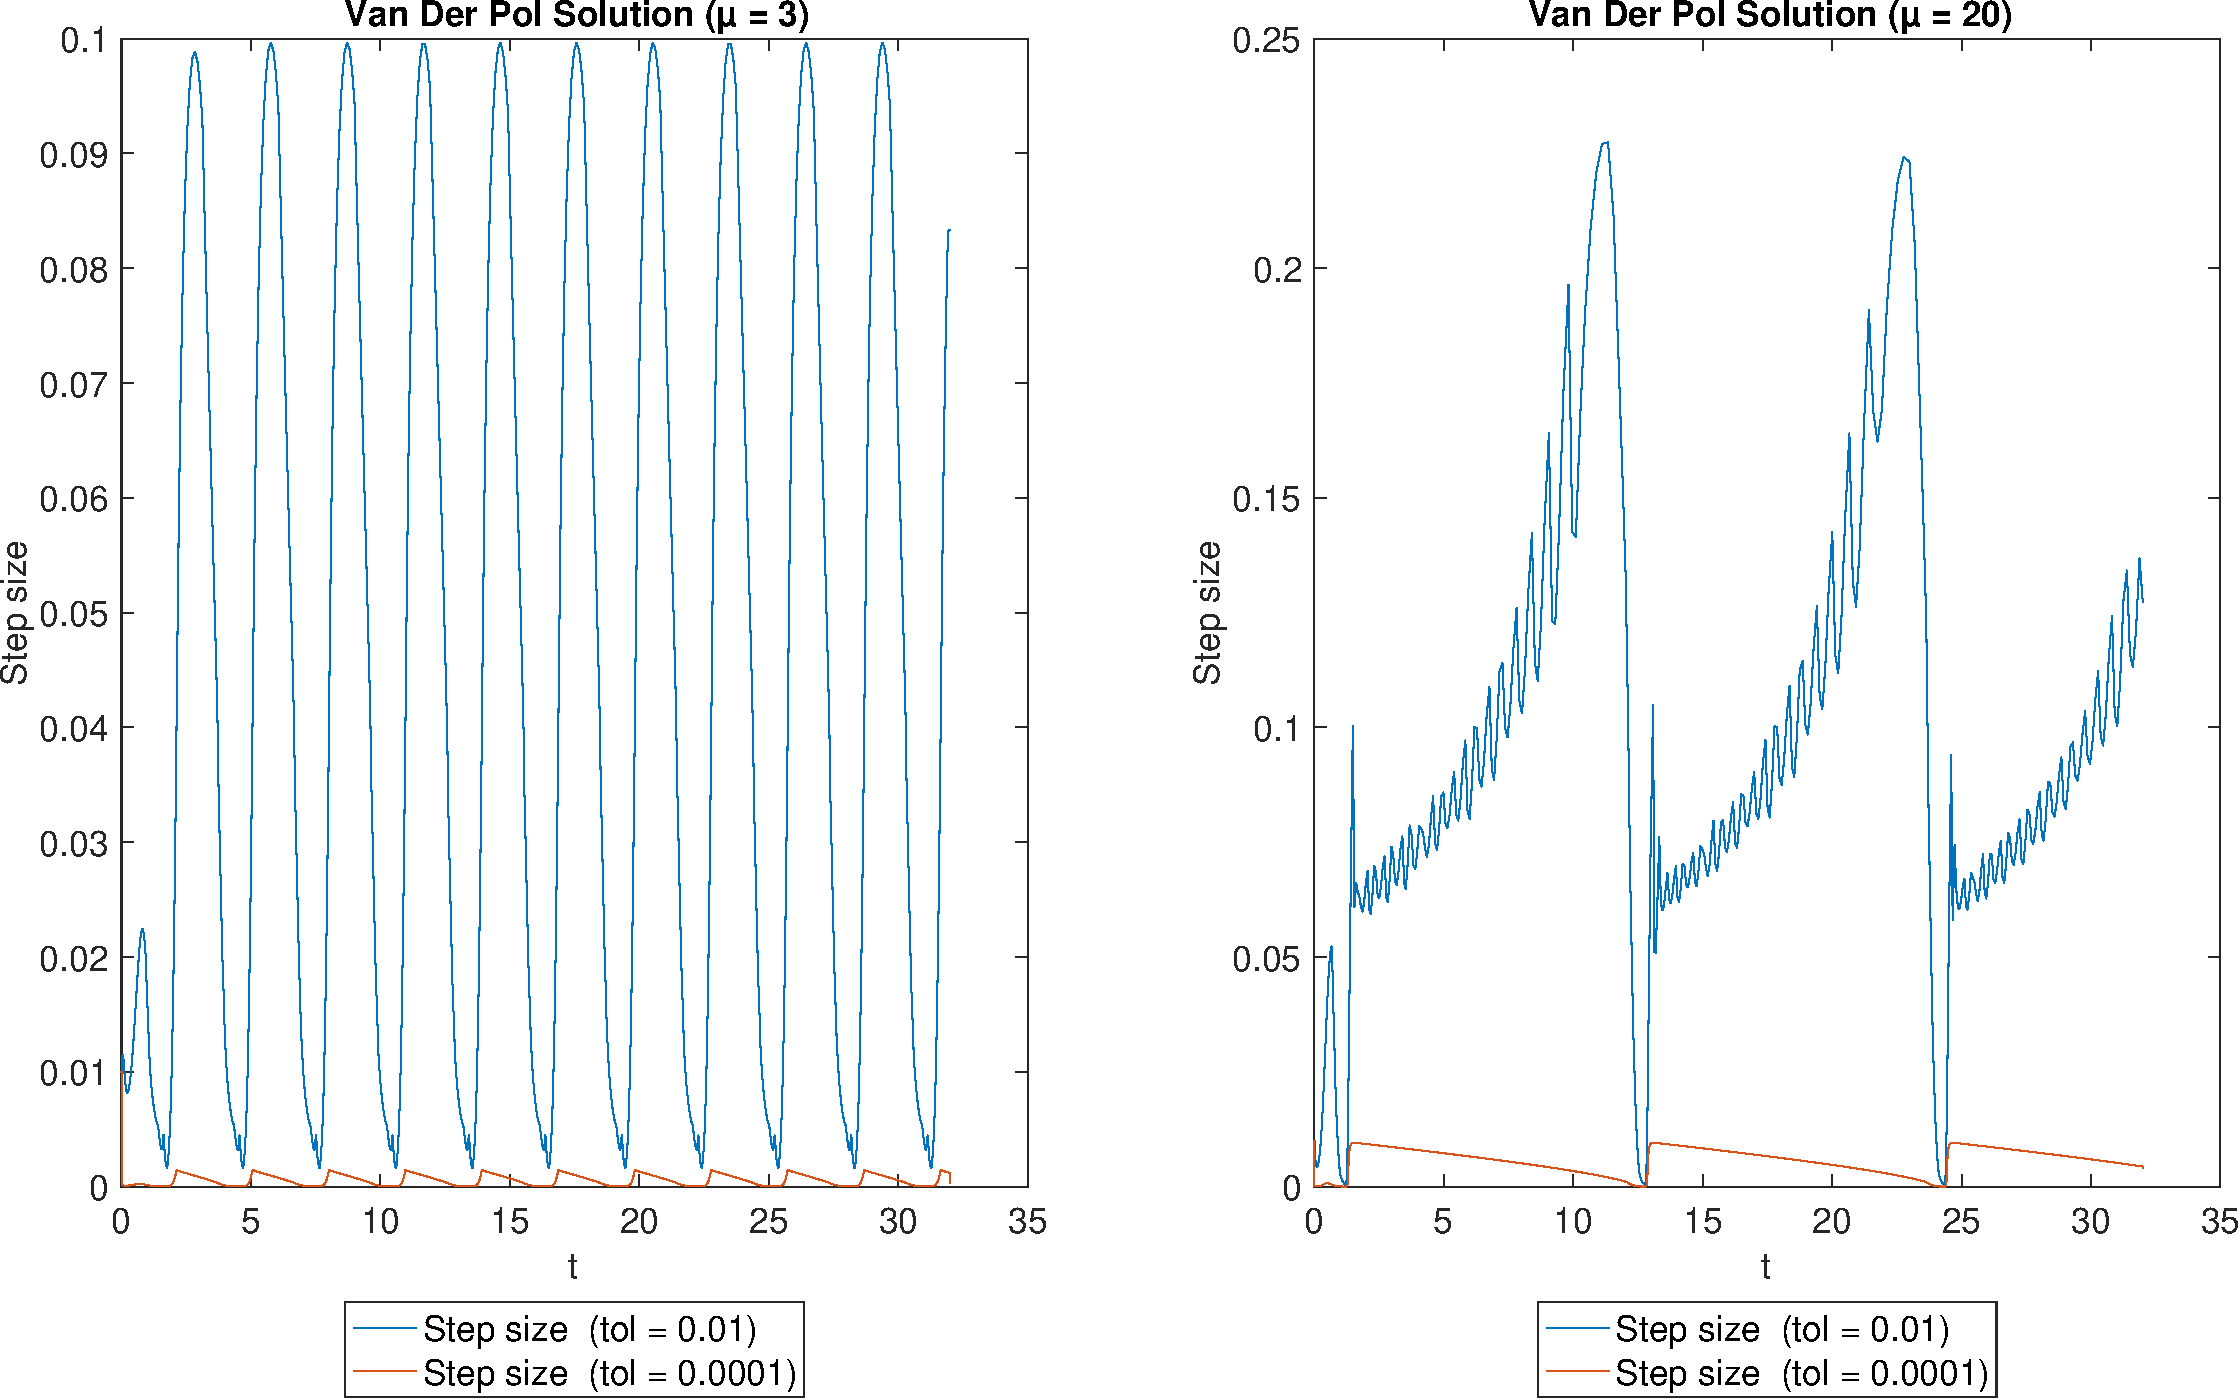
\includegraphics[width=1\linewidth]{plots/5_4b.pdf}
   \caption{}
   \label{fig:5_4b}
\end{subfigure}

\caption[Two numerical solutions]{(a) Solved $x_1$ and $x_2$ of the Van der Pol using classical Runge-Kutta with adaptive step size. (b) Corresponding step sizes.}
\end{figure}



\subsection{Discussion of interface}
In this sections we have seen the classical Runge-Kutta method, where the calculation of $x_{k+1}$ is done using 4 intermediate steps. Since the classical Runge-Kutta method is a very specific case of the general Runge-Kuta methods, it seems obvious to implement the more general family. That is what I did originally. But to show the classical Runge-Kutta more explicitly it was implemented directly\\
It was implemented in a similar fashion to MATLAB’s ode45 and ode15s for easy switching between solvers.
